\documentclass[main]{subfiles}
\begin{document}

%@@@@@@@@@@@@@@@@@@@@@@@@@@@@@@
% Main Topics: optimization problems, polyhedra, convexity.
% Optimization problems in finite dimensional space, basic definitions and
% examples of optimization problems: 21.09.2017
% tutorial - definitions, classifications of optimization problems and
% complexity theory: 22.09.2017
% author: Vanessa Leite

\section{Introduction}

\subsection{Complexity Theory - short revision}
Definition: an algorithm is a finite list of instructions. The running time of
an algorithm is the number of operations needed to complete it.

\paragraph{Simplifications}
\begin{itemize}
\item We measure the ``complexity'' of an algorithm with respect to the length
of the input, $n$.
$T_{A}(n)$ = complexity of the algorithm = worst case for same input size =
calculated/defined as the maximum over all inputs of length $n$.

\item We are only interested in how $T_{A}(n)$ increases w.r.t. $n$. \\
$T_{A}(n) = O(n)$: ``linear'' \\
$T_{A}(n) = O(n^k)$: ``polynomial'' \\
$T_{A}(n) = O(2^n)$: ``exponential'' \\

\item We assume that every operation of the algorithm requires the same cost
(``unit cost model'').
\end{itemize}

\subparagraph{Note}
We need to assume that the number of bits of any stored member must be bounded
by a (constant) multiple of the number of bits of the largest input value.
Example: if $a \in \mathbb{Z}$ is part of the input, its input size is $O(log
|a|)$. An algorithm with running time of $O(a)$ is not polynomial-time!
$(O(e^{log a})$: ``pseudo polynomial time'' $\rightarrow O((log m \times
A_{ij}) \times m \times n)$.

\subsubsection{Decision Problems}
Let $\Sigma = \{0,1\}$ and $\Sigma^{*}$ be a finite binary sequences (sequences
on $\Sigma$). We assume that all problems are encoded as elements of
$\Sigma^{*}$.

Definition \emph{$\mathcal{P}$ problems}: For a set $S \subseteq \Sigma^{*}$,
the decision problem defined by $S$ is the problem wether a given $x \in
\Sigma^{*}$ is in $S$ or not.

It is a polynomial-time solvable ($S \in \mathcal{P}$) if there exists an
algorithm $\mathcal{A}$ s.t. $\forall x \in \Sigma^{*}, \mathcal{A}(x) = 1 \iff
x \in S$.

If you can solve a decision problem, usually you can solve the optimization
problem.

Definition \emph{$\mathcal{NP}$ problems}: The decision problem defined by $S
\subseteq \Sigma^{*}$ is in $\mathcal{NP}$ if there is a polynomial time
algorithm $\mathcal{A}: \Sigma^{*} \times \Sigma^{*} \mapsto \{0,1\}$ and a
polynomial $p$, s.t.:
\begin{itemize}
\item $ \forall x \in S, \exists y \in \Sigma^{*}$ s.t. $|y| \in O(p(|x|)$ and
$\mathcal{A}(x,y) = 1$
\item $ \forall x \in S, \forall y in \Sigma^{*}, \mathcal{A}(x,y) = 0$
\end{itemize}

Example of $\mathcal{P}$ problems: Let $G=(V,E)$ be an undirected graph. ``does
$G$ have a cycle?''; ``does $G$ have a perfect matching?''.
Example of $\mathcal{NP}$ problems: ``does there exist a cycle covering all
vertices (hamiltonian cycle)?''. This problem is easy to check, given a cycle,
if it covers all vertices, however, it is not that easy find the cycle.

\paragraph{NP-Hard vs NP-Complete}
A decision problem $S$ is reducible to $S' (S \subseteq pS') \iff$ there is a
function $f: \Sigma^{*} \mapsto \Sigma^{*}$ compatible in polynomial s.t. $x
\in S \iff f(x) \in S'$.

\subparagraph{Lemma}
Let $S, S'$ be decision problems. If $S' \in \mathcal{P}$ (is polynomial-time
solvable). Then, $S \subseteq pS' \Rightarrow S \in \mathcal{P}$.

Definition NP-Complete: A decision problem is called NP-complete if $S \in
\mathcal{NP}$ and $\forall S' \in \mathcal{NP}, S' \subseteq pS$. If you have a
solution for $S$, you could solve all other $S$ problems in polynomial time.

Definition NP-Hard: A decision problem $S$ is NP-Hard if $\forall S' \in
\mathcal{NP}, S' \subseteq pS$.


\subsection{Optimization problems in finite dimensional space}
Definition: Let $f: \mathbb{R}^{n} \rightarrow \mathbb{R}$ be a function.
$dom(f) = \{ x \in \mathbb{R}^{n} \mid \left| f(x) \right| < \infty \}$.

We need a function to optimize. An optimization problem is of the form: 

\begin{equation*}
\begin{aligned}
& \underset{\mathbf{x \in \mathcal{F}}}{\text{min/max}}
& & f(\mathbf{x})
\end{aligned}
\label{eq:sampleOptimizationProblem}
\end{equation*}

Where $\mathcal{F} \subseteq \mathbb{R}^{n}$ is the feasible domain given
implicitly or by a ``membership oracle''. The function
$\mathcal{F}: \mathbb{R}^{n} \leftarrow \mathbb{R}$ is presented implicitly
(i.e., is a domain you can't describe) or by an ``evaluation oracle'', for
instance, given by a query: $x \in \mathbb{R}^{n}$: true ($x \in \mathcal{F}$)
or false ($x \notin \mathcal{F}$).

\textbf{Implicitly} means that you need evaluate by a given point; continuum spectrum of points can be scaled and produce a minimum nore negative than any natural.

\paragraph{What does $\displaystyle \min_{x \in \mathcal{F}} f(x)$ mean for us?}
This problem can be assigned to one of three meanings:
\begin{itemize} \label{items:optimization-conclusions}
\item nothing: the problem is \emph{infeasible}; it means that the domain is
empty, i.e., $\mathcal{F} = \emptyset$, there is nothing to optimize.
\item the problem is \emph{unbounded}, i.e., there exists a sequence of
points $x^{1}, x^{2}, \dots \in \mathcal{F}$ and $\forall n \in \mathbb{N},
f(x^{1}) < -n \Rightarrow lim_{i \rightarrow \infty} f(x^{i}) = -\infty$.
There exists a sequence of points that for each natural number, $f(x^{i} < -n$,
so we cannot bound the sequence.
\item the problem has an \emph{optimal solution}, i.e., $\exists x^{*} \in
\mathcal{F}$ such that $f(x^{*}) \leq f(z) \forall z \in \mathcal{F}$.
\end{itemize}

\paragraph{Target of the course}
Derive conclusions( meanings from above~\ref{items:optimization-conclusions}) for optimization
problem $\displaystyle \min_{x \in \mathcal{F}} f(x)$ and give ideally a proof
that our conclusion is correct. It is necessary to proof (find a proof) to hold
the conclusions. What to do when the se $\mathcal{F}$ is empty? It is necessary
a mathematical theory.


\subsection{Basic definitions}
\todo[inline]{organize the enumeration of figures in the text}
\begin{itemize}
\item A \emph{half space} is a set of the form $\{ x \in \mathbb{R}^{n} \mid
a^{T} x \leq \alpha \}$ for $a \in \mathbb{R}^{n}, \alpha \in \mathbb{R}$.
\subitem A \emph{half space rational} is a set of the form $\{ x \in
\mathbb{R}^{n} \mid a^{T} x \leq \alpha \}$ for $a \in \mathbb{Q}^{n}, \alpha
\in \mathbb{Q}$. In this case the boundary is a rational line.

\item A \emph{polyhedron} is the intersection of a \textbf{finite} number of
halfspaces (Figure~\ref{fig:polyhedron}). The intersection of halfspaces gives a
region of finite points. In this case, it is called \emph{polytope}: a bounded
polyhedron. We need to use geometry and algebric forms. In algebric form:
$\mathcal{P} = \{ x \in \mathbb{R}^{n} \mid Ax \leq b \} = \{ x \in
\mathbb{R}^{n} \mid a_{1}^{T}x \leq b_{1}, \dots, a_{n}^{T}x \leq b_{n} \}$
where $A \in \mathbb{R}^{m \times n}, b \in \mathbb{R}^{m}$. $A$ is a matrix
and $Ax \leq b$ represents each row of $A$.
\subitem Rational polyhedron: $A \in \mathbb{Q}^{ m \times n}, b \in
\mathbb{Q}^{m}$.
\subitem one half space is also a polyhedron.
\subitem all points inside a polyhedron are called feasible.
\subitem $Ax \leq b$ represents the multplication of the rows of $A$ with $x$. This is less equal than a value in $b$.
\todo[inline]{add a graphical representation of this subitem}

\item A set $\mathcal{Q}$ is \emph{convex} (Figure~\ref{fig:convex-set}) if
$\forall x, y \in \mathcal{Q}$ and $\lambda \in (0,1)$ then $\lambda x +
(1 - \lambda)y \in \mathcal{Q}$.

\item A function $f$ is \emph{linear} if $f(x) = c^{T}x$ for $c \in
\mathbb{R}^{n}$.

\item A function $f$ is \emph{convex} if $f: \mathbb{R}^{n} \rightarrow
\mathbb{R} \Rightarrow \emptyset \neq dom(\mathcal{F})$ is a convex set and
$f(\lambda x + (1-\lambda)y) \leq \lambda (f(x)) + (1-\lambda)(f(y)) \forall
x, y \in dom(\mathcal{F})$ and $\forall \lambda \in (0,1)$.

\item A function $f$ is \emph{strictly convex} if $f(\lambda x + (1-\lambda)y)
< \lambda (f(x)) + (1-\lambda)(f(y)) \forall x, y \in dom(\mathcal{F})$ and
$\forall \lambda \in (0,1)$.

\item lef $f$ be continuously differentiable, then $f$ is convex if, and only
if, $f(y) \geq f(x) + \Delta f(x)^{T}(yx) \forall y,x \in dom(f)$. And strictly
convex if, and only if, $f(y) > f(x) + \Delta f(x)^{T}(yx) \forall y,x \in
dom(f)$ and $y \neq x$.

\item If $f$ is twice differentiable, then $f$ is convex if, and only if,
$\Delta^{2} f(x) \geq 0, \forall x \in dom(f)$ (positive semidefinite).
\end{itemize}

\begin{figure}
  \label{fig:polyhedron}
  \caption{A polyhedron/polytope.}
  \centering
    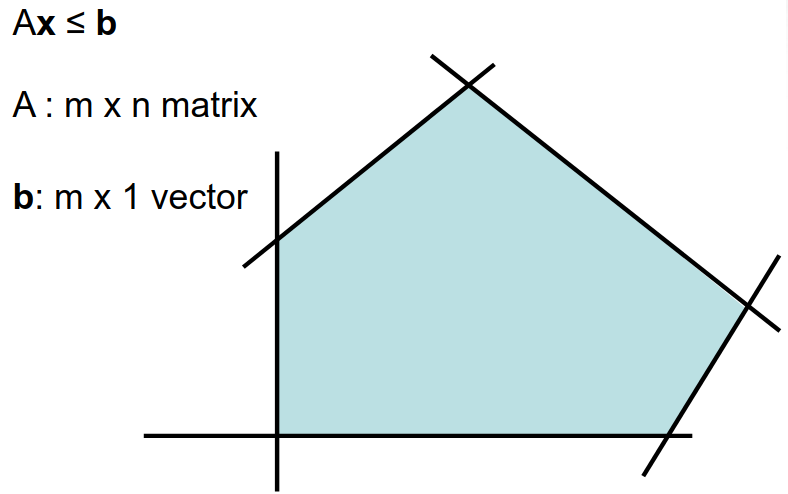
\includegraphics[width=0.5\textwidth]{imgs/polyhedron.png}
\end{figure}

\begin{figure}
  \label{fig:convex-set}
  \caption{Convex and non-convex set.}
  \centering
    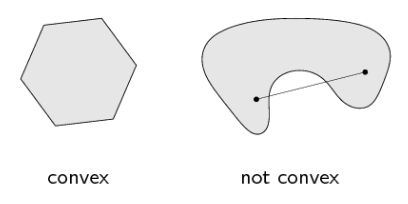
\includegraphics[width=0.5\textwidth]{imgs/convex-set.png}
\end{figure}


\paragraph{Convex set}
Given vectors $(x^{1}, \dots, x^{t} \in \mathbb{R}^{n})$ the convex hull of
this vectors are defined as $conv(x^{1}, \dots, x^{t}):= \{ x \in
\mathbb{R}^{n} \mid \exists \lambda_{1}, \dots, \lambda_{t} \geq 0 \}$ such
that $\mathds{1}^{T} \lambda = 1$ ( or $\sum_{i=1}^{t} \lambda_{i} = 1$):
$x = \sum_{i=1}^{t} \lambda_{i} x^{i}$.

\subparagraph{Note}
$conv(x^{1}, \dots, x^{t}) = \{ x \in \mathbb{R}^{n} \mid x = \sum_{i=1}^{t}
\lambda_{i} x^{i}, \lambda \geq 0, \sum \lambda = 1 \}$ is a special case of a
polyhedron (bounded polyhedron) and every bounded polyhedron is of this form.

\subparagraph{Lemma}
\begin{enumerate}
\item \label{item:polyhedron-convex-set} a polyhedron is a convex set
\item \label{item:convex-hull-convex-set} $conv(x^{1}, \dots, x^{t})$ is a convex set
\end{enumerate}

\subparagraph{Proof of~\ref{item:polyhedron-convex-set}}
Let $\mathcal{P} = \{ x \in \mathbb{R}^{n} \mid Ax \leq b\}$. Let $x,y \in
\mathcal{P}, \lambda \in (0,1)$. Show $\lambda x + (1 - \lambda) y \in
\mathcal{P}$.

\begin{gather*}
A [\lambda x + (1-\lambda)y ] = \lambda Ax + (1-\lambda)Ay \\
 \lambda Ax \leq \lambda b \  \text{and}\  (1-\lambda)Ay \leq (1-\lambda) b \\
 \lambda Ax + (1-\lambda)Ay \leq \lambda b + (1-\lambda) b = b \\
 \Rightarrow \lambda x + (1-\lambda)y \in \mathcal{P}.
\end{gather*}

\subparagraph{Proof of~\ref{item:polyhedron-convex-set}}
Let $x^{1}, \dots, x^{t} \in \mathbb{R}^{n}$. Let $x,y \in conv(x^{1}, \dots,
x^{t})\ \text{and} \ 0 < \lambda < 1$. Show $\lambda x + (1-\lambda)y \in
conv(x^{1}, \dots, x^{t})$.

$x$ lies in $conv(x^{1}, \dots, x^{t})$. What does that means? That implies
$x = \sum_{i=1}^{t} \mu_{i} x^{i}, \mu_{i} \geq 0 \forall i$ and 
$y = \sum_{i=1}^{t} \sigma_{i} x^{i}, \sigma_{i} \geq 0 \forall i$

\begin{gather*}
\lambda x + (1-\lambda)y = \sum_{i=1}^{t} \lambda \mu_{i} x^{i} +
\sum_{i=1}^{t} (1-\lambda) \sigma_{i} x^{i} \\
= \sum_{i=1}^{t} (\lambda \mu_{i} + (1-\lambda) \sigma_{i}) x^{i} \\
\tau_{i} = (\lambda \mu_{i} + (1-\lambda) \sigma_{i}), \tau_{i} \geq 0, \forall i \\
= \sum_{i=1}^{t} \tau_{i} = \sum_{i=1}^{t} (\lambda \mu_{i} + (1-\lambda) \sigma_{i}) \\
= \lambda \sum_{i=1}^{t} \mu_{i} + (1-\lambda) \sum_{i=1}^{t} \sigma_{i} \\
\sum_{i=1}^{t} \mu_{i} = 1 \ \text{and} \ \sum_{i=1}^{t} \sigma_{i} = 1 \\
= \lambda + (1-\lambda) = 1
\end{gather*}

\subsection{Classification of Optimization Problems}
Definition of optimization problem: For $f: \mathbb{R}^{n} \mapsto \mathbb{R}$
(any function), solve $\displaystyle \min_{x \in \mathcal{F}} f(x)$ (objective
value) or $\displaystyle \argmin_{x \in \mathcal{F}} f(x)$ (value of $x$ that
minimize $f(x)$).
\subparagraph{Note}
$\displaystyle \max_{x \in \mathcal{F}} f(x) = \min_{x \in \mathcal{F}} -f(x)$

\begin{itemize}
\item \emph{linear optimization problem}: given $A \in \mathcal{Q}^{m \times n}, b \in
\mathcal{Q}^{m}, c \in \mathcal{Q}^{n}$. $\displaystyle \min_{x \in
\mathcal{P}} c^{T}x$ where $\mathcal{P}$ is a polyhedron defined by $\{ x \in
\mathcal{R}^{n} \mid x_{i} \geq 0 \forall i, Ax = b \}$ or $\displaystyle
\max_{x \in \mathcal{P}} c^{T}x$ where $\mathcal{P} = \{ x \in
\mathcal{R}^{n} \mid Ax \leq b \}$ \\
$c^{T}x$ is the objective (linear) function. \\
$Ax \leq b$ is the constraint/feasible region.\\
Can be solved quickly and in polinomial time.

\subitem \emph{integer linear optimization problem} (Figure~\ref{fig:ILP}).
$max/min \{ c^{T}x \mid Ax \leq b, x \in \mathbb{Z}^{n} \}$.
Solve a integer optimization problem can lead to a better result than just
round linear solutions.

\begin{figure}
  \label{fig:ILP}
  \caption{ILP}
  \centering
    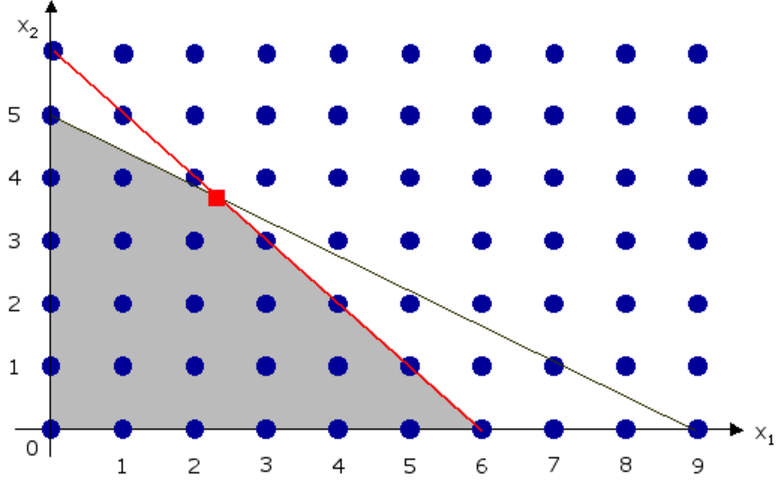
\includegraphics[width=0.5\textwidth]{imgs/ILP.png}
\end{figure}

\subitem \emph{mixed integer linear optimization problem}
$max/min \{ c^{T}x \mid Ax \leq b, x \in \mathbb{Z}^{n-d} \times
\mathbb{R}^{d} \}$.

\item \emph{convex optimization problem}: $\mathcal{F}$ is a convex set, $f:
\mathcal{R}^{n} \rightarrow \mathcal{R}$ is a convex function and $\mathcal{F}
\subseteq dom(f)$\\
$f(x)$ convex and $\mathcal{F}$ convex set. $\forall x, y \in \mathbb{R}^{n},
\lambda \in [0,1], f(\lambda x + (1-\lambda)y) \leq \lambda f(x) + (1-\lambda)
f(y)$. $\forall x,y \in \mathcal{F}, \lambda x + (1-\lambda)y \in \mathcal{F}$.


\todo[inline]{Example of implicitly: knapsack problem: collection are all
feasible solutions of knapsack problem.}

\item \emph{combinatorial optimization problem}: given finite groundset $\mathcal{E}$
and a collection $\mathcal{I}$ of subsets of $\mathcal{E}$ (tipically,
implicitly given: you cannot write it down).
For $c: \mathcal{E} \mapsto \mathcal{R}$ find a member in the collection $(I
\in \mathcal{I})$ such that $\sum_{i \in I} c_{i}$ is minimal/maximal.
Example: $G = (V, E), E \subseteq V \times V$
$S \subseteq V$ stable implies that for all pairs in $S (\forall i,j \in S)$,
the corresponding edge $i,j$ is not present $(i \neq j, (i,j) \notin E)$.
Groundset: $V$ \\
$\mathcal{I} \subseteq 2^{V}$ \\
$I \in \mathcal{I} \iff I$ is stable in $G$ (implicitly given) \\
$c: V \mapsto \mathcal{R}$; suppose $c(v) = 1, \forall c \in V$ \\
find a maximal (w.r.t. cardinality) stable set in $G$

\item \emph{general integer optimization problem}: \\
$\displaystyle \max_{x \in \mathcal{P} \cap \mathbb{Z}^{n}} c^{T}x,
\mathcal{P} = \{ x \in \mathbb{R}^{n} \mid Ax \leq b \}$
or 
$\displaystyle \min_{x \in \mathcal{P} \cap \mathbb{Z}^{n}} c^{T}x,
\mathcal{P} = \{ x \in \mathbb{R}^{n} \mid x_{i} \geq 0 \forall i, Ax = b \}$

\end{itemize}



\end{document}